

\section{Les axes XPath}

\begin{frame}{Les axes dans XPath (déf. W3C)}

\begin{tabular}{| l | p{8cm} |}
\hline
Axis name & Semantics \\
\hline
\hline
child & Selects all children of the current node (défaut)\\
\hline
attribute & Selects all attributes of the current node \\
\hline
ancestor & Selects all ancestors of the current node \\
\hline
ancestor-or-self & Selects all ancestors of the current node and the current node itself \\
\hline
descendant & Selects all descendants  of the current node \\
\hline
descendant-or-self & Selects all descendants of the current node and the current node itself \\
\hline
following & Selects everything in the document defined after the closing tag of the current node \\
\hline
following-sibling & Selects all siblings after the current node \\
\hline
namespace & Selects all namespace nodes of the current node \\
\hline
parent & Selects the parent of the current node \\
\hline
preceding & Selects everything in the document that is defined before the start tag of the current node \\
\hline
preceding-sibling & Selects all siblings before the current node \\
\hline
self & Selects the current node \\
\hline
\end{tabular}

\end{frame}



\begin{frame}{Illustration\,: un document XML}


\lstinputlisting[basicstyle=\small, language=XML,breaklines=true, numbers=left, caption={Fichier twobooks.xml}]{codes/twobooks.xml}

\begin{exoblock}
Quelle est la forme arborescente (DOM) de ce document\,?
\end{exoblock}

\end{frame}


\begin{frame}{Quelques axes en exemple}

Prenons l'exemple de l'arbre DOM suivant\,:

\medskip


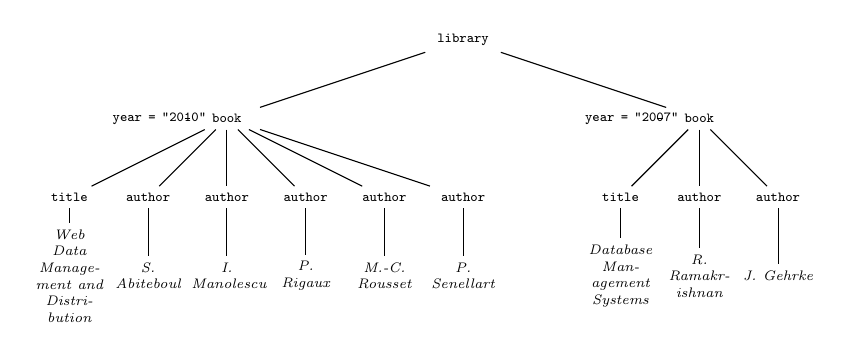
\begin{tikzpicture}[auto]
\tiny
  \tikzstyle{emptyStyle}=[text width=0.9cm, text centered]
  \tikzstyle{red}=[rounded corners=1mm,thick,draw=red!75,fill=red!20,text width=0.9cm, text centered]
  \tikzstyle{DarkViolet}=[rounded corners=1mm,thick,draw=DarkViolet!75,fill=DarkViolet!20,minimum size=7mm,text width=0.8cm, text centered]
  \tikzstyle{green}=[rounded corners=1mm,thick,draw=DarkOliveGreen!75,fill=DarkOliveGreen!20,minimum size=7mm,text width=0.8cm, text centered]
  \tikzstyle{cyan}=[rounded corners=1mm,thick,draw=DarkCyan!75,fill=DarkCyan!20,minimum size=7mm,text width=0.8cm, text centered]
 \tikzstyle{every label}=[black]
  \tikzstyle{HotPink}=[rounded corners=1mm,thick,draw=HotPink!75,fill=HotPink!20,minimum size=7mm,text width=0.8cm, text centered]
  \tikzstyle{Olive}=[rounded corners=1mm,thick,draw=Olive!75,fill=Olive!20,minimum size=7mm,text width=0.9cm, text centered]
  \tikzstyle{indiaRed}=[rounded corners=1mm,thick,draw=indiaRed!75,fill=indiaRed!20,minimum size=7mm,text width=0.9cm, text centered]

  \begin{scope}
   % \node[emptyStyle](r) at (7,5) {Root};  
   %\node[emptyStyle](entete) at (3,4) {\texttt{$<?xml$ version $...>$}};
   %\draw[-] (r) -- (entete);
   \node[emptyStyle](library) at (7,4) {\verb?library?};
   % \draw[-] (r) -- (library);

    \node[emptyStyle](book1) at (4,3) {\verb?book?};
   \draw[-] (library) -- (book1);
   \node[emptyStyle](book2) at (10,3) {\verb?book?};
   \draw[-] (library) -- (book2);

    \node[emptyStyle](year1) at (3,3) {\verb?year = "2010"?};
   \draw[-] (book1) -- (year1);
    \node[emptyStyle](title1) at (2,2) {\verb?title?};
   \draw[-] (book1) -- (title1);
 \node[emptyStyle](texttitle1) at (2,1) {\it Web Data Management and Distribution};
   \draw[-] (title1) -- (texttitle1);
    \node[emptyStyle](author1) at (3,2) {\verb?author?};
   \draw[-] (book1) -- (author1);
   \node[emptyStyle](textauthor1) at (3,1) {\it S. Abiteboul};
   \draw[-] (author1) -- (textauthor1);
    \node[emptyStyle](author2) at (4,2) {\verb?author?};
   \draw[-] (book1) -- (author2);
   \node[emptyStyle](textauthor2) at (4,1) {\it I. Manolescu};
   \draw[-] (author2) -- (textauthor2);
    \node[emptyStyle](author3) at (5,2) {\verb?author?};
   \draw[-] (book1) -- (author3);
   \node[emptyStyle](textauthor3) at (5,1) {\it P. Rigaux};
   \draw[-] (author3) -- (textauthor3);
    \node[emptyStyle](author4) at (6,2) {\verb?author?};
   \draw[-] (book1) -- (author4);
   \node[emptyStyle](textauthor4) at (6,1) {\it M.-C. Rousset};
   \draw[-] (author4) -- (textauthor4);
    \node[emptyStyle](author5) at (7,2) {\verb?author?};
   \draw[-] (book1) -- (author5);
   \node[emptyStyle](textauthor5) at (7,1) {\it P. Senellart};
   \draw[-] (author5) -- (textauthor5);

    \node[emptyStyle](year2) at (9,3) {\verb?year = "2007"?};
   \draw[-] (book2) -- (year2);
    \node[emptyStyle](title2) at (9,2) {\verb?title?};
   \draw[-] (book2) -- (title2);
 \node[emptyStyle](texttitle2) at (9,1) {\it Database Management Systems};
   \draw[-] (title2) -- (texttitle2);
    \node[emptyStyle](author1prime) at (10,2) {\verb?author?};
   \draw[-] (book2) -- (author1prime);
   \node[emptyStyle](textauthor1prime) at (10,1) {\it R. Ramakrishnan};
   \draw[-] (author1prime) -- (textauthor1prime);
    \node[emptyStyle](author2prime) at (11,2) {\verb?author?};
   \draw[-] (book2) -- (author2prime);
   \node[emptyStyle](textauthor2prime) at (11,1) {\it J. Gehrke};
   \draw[-] (author2prime) -- (textauthor2prime);

\end{scope}

\end{tikzpicture}


\end{frame}



\subsection{Child}

\begin{frame}{Quelques axes en exemple : \texttt{child}}

\texttt{child} : tous les enfants du n{\oe}ud courant.

\medskip


\texttt{child} est l'axe par défaut, on peut l'omettre dans les expressions.


\bigskip

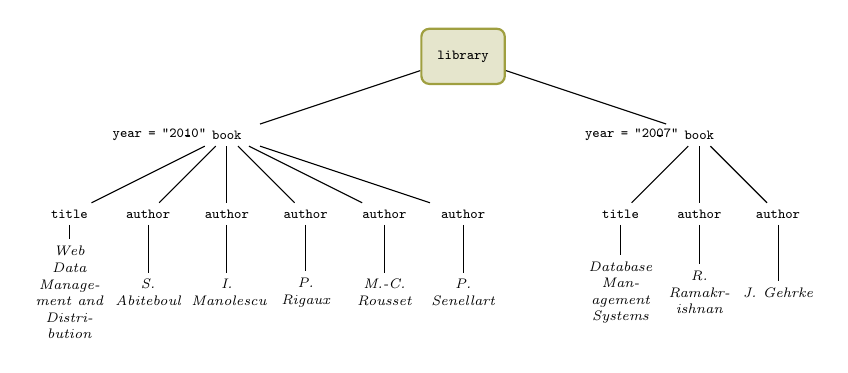
\begin{tikzpicture}[auto]
\tiny
  \tikzstyle{emptyStyle}=[text width=0.9cm, text centered]
  \tikzstyle{red}=[rounded corners=1mm,thick,draw=red!75,fill=red!20,text width=0.9cm, text centered]
  \tikzstyle{DarkViolet}=[rounded corners=1mm,thick,draw=DarkViolet!75,fill=DarkViolet!20,minimum size=7mm,text width=0.8cm, text centered]
  \tikzstyle{green}=[rounded corners=1mm,thick,draw=DarkOliveGreen!75,fill=DarkOliveGreen!20,minimum size=7mm,text width=0.8cm, text centered]
  \tikzstyle{cyan}=[rounded corners=1mm,thick,draw=DarkCyan!75,fill=DarkCyan!20,minimum size=7mm,text width=0.8cm, text centered]
 \tikzstyle{every label}=[black]
  \tikzstyle{HotPink}=[rounded corners=1mm,thick,draw=HotPink!75,fill=HotPink!20,minimum size=7mm,text width=0.8cm, text centered]
  \tikzstyle{noeudcourant}=[rounded corners=1mm,thick,draw=Olive!75,fill=Olive!20,minimum size=7mm,text width=0.9cm, text centered]
  \tikzstyle{indiaRed}=[rounded corners=1mm,thick,draw=indiaRed!75,fill=indiaRed!20,minimum size=7mm,text width=0.9cm, text centered]

  \begin{scope}
   % \node[emptyStyle](r) at (7,5) {Root};  
   %\node[emptyStyle](entete) at (3,4) {\texttt{$<?xml$ version $...>$}};
   %\draw[-] (r) -- (entete);
   \node[noeudcourant](library) at (7,4) {\verb?library?};
   % \draw[-] (r) -- (library);

    \node[emptyStyle](book1) at (4,3) {\verb?book?};
   \draw[-] (library) -- (book1);
   \node[emptyStyle](book2) at (10,3) {\verb?book?};
   \draw[-] (library) -- (book2);

    \node[emptyStyle](year1) at (3,3) {\verb?year = "2010"?};
   \draw[-] (book1) -- (year1);
    \node[emptyStyle](title1) at (2,2) {\verb?title?};
   \draw[-] (book1) -- (title1);
 \node[emptyStyle](texttitle1) at (2,1) {\it Web Data Management and Distribution};
   \draw[-] (title1) -- (texttitle1);
    \node[emptyStyle](author1) at (3,2) {\verb?author?};
   \draw[-] (book1) -- (author1);
   \node[emptyStyle](textauthor1) at (3,1) {\it S. Abiteboul};
   \draw[-] (author1) -- (textauthor1);
    \node[emptyStyle](author2) at (4,2) {\verb?author?};
   \draw[-] (book1) -- (author2);
   \node[emptyStyle](textauthor2) at (4,1) {\it I. Manolescu};
   \draw[-] (author2) -- (textauthor2);
    \node[emptyStyle](author3) at (5,2) {\verb?author?};
   \draw[-] (book1) -- (author3);
   \node[emptyStyle](textauthor3) at (5,1) {\it P. Rigaux};
   \draw[-] (author3) -- (textauthor3);
    \node[emptyStyle](author4) at (6,2) {\verb?author?};
   \draw[-] (book1) -- (author4);
   \node[emptyStyle](textauthor4) at (6,1) {\it M.-C. Rousset};
   \draw[-] (author4) -- (textauthor4);
    \node[emptyStyle](author5) at (7,2) {\verb?author?};
   \draw[-] (book1) -- (author5);
   \node[emptyStyle](textauthor5) at (7,1) {\it P. Senellart};
   \draw[-] (author5) -- (textauthor5);

    \node[emptyStyle](year2) at (9,3) {\verb?year = "2007"?};
   \draw[-] (book2) -- (year2);
    \node[emptyStyle](title2) at (9,2) {\verb?title?};
   \draw[-] (book2) -- (title2);
 \node[emptyStyle](texttitle2) at (9,1) {\it Database Management Systems};
   \draw[-] (title2) -- (texttitle2);
    \node[emptyStyle](author1prime) at (10,2) {\verb?author?};
   \draw[-] (book2) -- (author1prime);
   \node[emptyStyle](textauthor1prime) at (10,1) {\it R. Ramakrishnan};
   \draw[-] (author1prime) -- (textauthor1prime);
    \node[emptyStyle](author2prime) at (11,2) {\verb?author?};
   \draw[-] (book2) -- (author2prime);
   \node[emptyStyle](textauthor2prime) at (11,1) {\it J. Gehrke};
   \draw[-] (author2prime) -- (textauthor2prime);
\end{scope}
\end{tikzpicture}
\end{frame}


\begin{frame}{Quelques axes en exemple : \texttt{child}}
\texttt{child} : tous les enfants du n{\oe}ud courant.


\bigskip

\begin{tikzpicture}[auto]
\tiny
  \tikzstyle{emptyStyle}=[text width=0.9cm, text centered]
  \tikzstyle{red}=[rounded corners=1mm,thick,draw=red!75,fill=red!20,text width=0.9cm, text centered]
  \tikzstyle{DarkViolet}=[rounded corners=1mm,thick,draw=DarkViolet!75,fill=DarkViolet!20,minimum size=7mm,text width=0.8cm, text centered]
  \tikzstyle{green}=[rounded corners=1mm,thick,draw=DarkOliveGreen!75,fill=DarkOliveGreen!20,minimum size=7mm,text width=0.8cm, text centered]
  \tikzstyle{cyan}=[rounded corners=1mm,thick,draw=DarkCyan!75,fill=DarkCyan!20,minimum size=7mm,text width=0.8cm, text centered]
 \tikzstyle{every label}=[black]
  \tikzstyle{HotPink}=[rounded corners=1mm,thick,draw=HotPink!75,fill=HotPink!20,minimum size=7mm,text width=0.8cm, text centered]
  \tikzstyle{noeudcourant}=[rounded corners=1mm,thick,draw=Olive!75,fill=Olive!20,minimum size=7mm,text width=0.9cm, text centered]
  \tikzstyle{indiaRed}=[rounded corners=1mm,thick,draw=indiaRed!75,fill=indiaRed!20,minimum size=7mm,text width=0.9cm, text centered]

  \begin{scope}
   % \node[emptyStyle](r) at (7,5) {Root};  
   %\node[emptyStyle](entete) at (3,4) {\texttt{$<?xml$ version $...>$}};
   %\draw[-] (r) -- (entete);
   \node[noeudcourant](library) at (7,4) {\verb?library?};
   %\draw[-] (r) -- (library);

    \node[indiaRed](book1) at (4,3) {\verb?book?};
   \draw[-] (library) -- (book1);
   \node[indiaRed](book2) at (10,3) {\verb?book?};
   \draw[-] (library) -- (book2);

    \node[emptyStyle](year1) at (3,3) {\verb?year = "2010"?};
   \draw[-] (book1) -- (year1);
    \node[emptyStyle](title1) at (2,2) {\verb?title?};
   \draw[-] (book1) -- (title1);
 \node[emptyStyle](texttitle1) at (2,1) {\it Web Data Management and Distribution};
   \draw[-] (title1) -- (texttitle1);
    \node[emptyStyle](author1) at (3,2) {\verb?author?};
   \draw[-] (book1) -- (author1);
   \node[emptyStyle](textauthor1) at (3,1) {\it S. Abiteboul};
   \draw[-] (author1) -- (textauthor1);
    \node[emptyStyle](author2) at (4,2) {\verb?author?};
   \draw[-] (book1) -- (author2);
   \node[emptyStyle](textauthor2) at (4,1) {\it I. Manolescu};
   \draw[-] (author2) -- (textauthor2);
    \node[emptyStyle](author3) at (5,2) {\verb?author?};
   \draw[-] (book1) -- (author3);
   \node[emptyStyle](textauthor3) at (5,1) {\it P. Rigaux};
   \draw[-] (author3) -- (textauthor3);
    \node[emptyStyle](author4) at (6,2) {\verb?author?};
   \draw[-] (book1) -- (author4);
   \node[emptyStyle](textauthor4) at (6,1) {\it M.-C. Rousset};
   \draw[-] (author4) -- (textauthor4);
    \node[emptyStyle](author5) at (7,2) {\verb?author?};
   \draw[-] (book1) -- (author5);
   \node[emptyStyle](textauthor5) at (7,1) {\it P. Senellart};
   \draw[-] (author5) -- (textauthor5);

    \node[emptyStyle](year2) at (9,3) {\verb?year = "2007"?};
   \draw[-] (book2) -- (year2);
    \node[emptyStyle](title2) at (9,2) {\verb?title?};
   \draw[-] (book2) -- (title2);
 \node[emptyStyle](texttitle2) at (9,1) {\it Database Management Systems};
   \draw[-] (title2) -- (texttitle2);
    \node[emptyStyle](author1prime) at (10,2) {\verb?author?};
   \draw[-] (book2) -- (author1prime);
   \node[emptyStyle](textauthor1prime) at (10,1) {\it R. Ramakrishnan};
   \draw[-] (author1prime) -- (textauthor1prime);
    \node[emptyStyle](author2prime) at (11,2) {\verb?author?};
   \draw[-] (book2) -- (author2prime);
   \node[emptyStyle](textauthor2prime) at (11,1) {\it J. Gehrke};
   \draw[-] (author2prime) -- (textauthor2prime);
\end{scope}
\end{tikzpicture}
\end{frame} 

\begin{frame}{Quelques axes en exemple : \texttt{child}}
\texttt{child} : tous les enfants du n{\oe}ud courant.

\bigskip

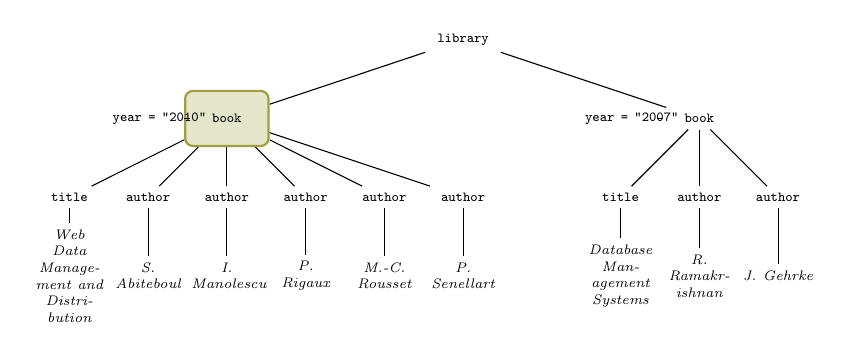
\begin{tikzpicture}[auto]
\tiny
  \tikzstyle{emptyStyle}=[text width=0.9cm, text centered]
  \tikzstyle{red}=[rounded corners=1mm,thick,draw=red!75,fill=red!20,text width=0.9cm, text centered]
  \tikzstyle{DarkViolet}=[rounded corners=1mm,thick,draw=DarkViolet!75,fill=DarkViolet!20,minimum size=7mm,text width=0.8cm, text centered]
  \tikzstyle{green}=[rounded corners=1mm,thick,draw=DarkOliveGreen!75,fill=DarkOliveGreen!20,minimum size=7mm,text width=0.8cm, text centered]
  \tikzstyle{cyan}=[rounded corners=1mm,thick,draw=DarkCyan!75,fill=DarkCyan!20,minimum size=7mm,text width=0.8cm, text centered]
 \tikzstyle{every label}=[black]
  \tikzstyle{HotPink}=[rounded corners=1mm,thick,draw=HotPink!75,fill=HotPink!20,minimum size=7mm,text width=0.8cm, text centered]
  \tikzstyle{noeudcourant}=[rounded corners=1mm,thick,draw=Olive!75,fill=Olive!20,minimum size=7mm,text width=0.9cm, text centered]
  \tikzstyle{indiaRed}=[rounded corners=1mm,thick,draw=indiaRed!75,fill=indiaRed!20,minimum size=7mm,text width=0.9cm, text centered]

  \begin{scope}
   % \node[emptyStyle](r) at (7,5) {Root};  
   %\node[emptyStyle](entete) at (3,4) {\texttt{$<?xml$ version $...>$}};
   %\draw[-] (r) -- (entete);
   \node[emptyStyle](library) at (7,4) {\verb?library?};
   % \draw[-] (r) -- (library);

    \node[noeudcourant](book1) at (4,3) {\verb?book?};
   \draw[-] (library) -- (book1);
   \node[emptyStyle](book2) at (10,3) {\verb?book?};
   \draw[-] (library) -- (book2);

    \node[emptyStyle](year1) at (3,3) {\verb?year = "2010"?};
   \draw[-] (book1) -- (year1);
    \node[emptyStyle](title1) at (2,2) {\verb?title?};
   \draw[-] (book1) -- (title1);
 \node[emptyStyle](texttitle1) at (2,1) {\it Web Data Management and Distribution};
   \draw[-] (title1) -- (texttitle1);
    \node[emptyStyle](author1) at (3,2) {\verb?author?};
   \draw[-] (book1) -- (author1);
   \node[emptyStyle](textauthor1) at (3,1) {\it S. Abiteboul};
   \draw[-] (author1) -- (textauthor1);
    \node[emptyStyle](author2) at (4,2) {\verb?author?};
   \draw[-] (book1) -- (author2);
   \node[emptyStyle](textauthor2) at (4,1) {\it I. Manolescu};
   \draw[-] (author2) -- (textauthor2);
    \node[emptyStyle](author3) at (5,2) {\verb?author?};
   \draw[-] (book1) -- (author3);
   \node[emptyStyle](textauthor3) at (5,1) {\it P. Rigaux};
   \draw[-] (author3) -- (textauthor3);
    \node[emptyStyle](author4) at (6,2) {\verb?author?};
   \draw[-] (book1) -- (author4);
   \node[emptyStyle](textauthor4) at (6,1) {\it M.-C. Rousset};
   \draw[-] (author4) -- (textauthor4);
    \node[emptyStyle](author5) at (7,2) {\verb?author?};
   \draw[-] (book1) -- (author5);
   \node[emptyStyle](textauthor5) at (7,1) {\it P. Senellart};
   \draw[-] (author5) -- (textauthor5);

    \node[emptyStyle](year2) at (9,3) {\verb?year = "2007"?};
   \draw[-] (book2) -- (year2);
    \node[emptyStyle](title2) at (9,2) {\verb?title?};
   \draw[-] (book2) -- (title2);
 \node[emptyStyle](texttitle2) at (9,1) {\it Database Management Systems};
   \draw[-] (title2) -- (texttitle2);
    \node[emptyStyle](author1prime) at (10,2) {\verb?author?};
   \draw[-] (book2) -- (author1prime);
   \node[emptyStyle](textauthor1prime) at (10,1) {\it R. Ramakrishnan};
   \draw[-] (author1prime) -- (textauthor1prime);
    \node[emptyStyle](author2prime) at (11,2) {\verb?author?};
   \draw[-] (book2) -- (author2prime);
   \node[emptyStyle](textauthor2prime) at (11,1) {\it J. Gehrke};
   \draw[-] (author2prime) -- (textauthor2prime);
\end{scope}
\end{tikzpicture}
\end{frame}


\begin{frame}{Quelques axes en exemple : \texttt{child}}
\texttt{child} : tous les enfants du n{\oe}ud courant.

\bigskip

\begin{tikzpicture}[auto]
\tiny
  \tikzstyle{emptyStyle}=[text width=0.9cm, text centered]
  \tikzstyle{red}=[rounded corners=1mm,thick,draw=red!75,fill=red!20,text width=0.9cm, text centered]
  \tikzstyle{DarkViolet}=[rounded corners=1mm,thick,draw=DarkViolet!75,fill=DarkViolet!20,minimum size=7mm,text width=0.8cm, text centered]
  \tikzstyle{green}=[rounded corners=1mm,thick,draw=DarkOliveGreen!75,fill=DarkOliveGreen!20,minimum size=7mm,text width=0.8cm, text centered]
  \tikzstyle{cyan}=[rounded corners=1mm,thick,draw=DarkCyan!75,fill=DarkCyan!20,minimum size=7mm,text width=0.8cm, text centered]
 \tikzstyle{every label}=[black]
  \tikzstyle{HotPink}=[rounded corners=1mm,thick,draw=HotPink!75,fill=HotPink!20,minimum size=7mm,text width=0.8cm, text centered]
  \tikzstyle{noeudcourant}=[rounded corners=1mm,thick,draw=Olive!75,fill=Olive!20,minimum size=7mm,text width=0.9cm, text centered]
  \tikzstyle{indiaRed}=[rounded corners=1mm,thick,draw=indiaRed!75,fill=indiaRed!20,minimum size=7mm,text width=0.9cm, text centered]

  \begin{scope}
   % \node[emptyStyle](r) at (7,5) {Root};  
   %\node[emptyStyle](entete) at (3,4) {\texttt{$<?xml$ version $...>$}};
   %\draw[-] (r) -- (entete);
   \node[emptyStyle](library) at (7,4) {\verb?library?};
   % \draw[-] (r) -- (library);

    \node[noeudcourant](book1) at (4,3) {\verb?book?};
   \draw[-] (library) -- (book1);
   \node[emptyStyle](book2) at (10,3) {\verb?book?};
   \draw[-] (library) -- (book2);

    \node[emptyStyle](year1) at (3,3) {\verb?year = "2010"?};
   \draw[-] (book1) -- (year1);
    \node[indiaRed](title1) at (2,2) {\verb?title?};
   \draw[-] (book1) -- (title1);
 \node[emptyStyle](texttitle1) at (2,1) {\it Web Data Management and Distribution};
   \draw[-] (title1) -- (texttitle1);
    \node[indiaRed](author1) at (3,2) {\verb?author?};
   \draw[-] (book1) -- (author1);
   \node[emptyStyle](textauthor1) at (3,1) {\it S. Abiteboul};
   \draw[-] (author1) -- (textauthor1);
    \node[indiaRed](author2) at (4,2) {\verb?author?};
   \draw[-] (book1) -- (author2);
   \node[emptyStyle](textauthor2) at (4,1) {\it I. Manolescu};
   \draw[-] (author2) -- (textauthor2);
    \node[indiaRed](author3) at (5,2) {\verb?author?};
   \draw[-] (book1) -- (author3);
   \node[emptyStyle](textauthor3) at (5,1) {\it P. Rigaux};
   \draw[-] (author3) -- (textauthor3);
    \node[indiaRed](author4) at (6,2) {\verb?author?};
   \draw[-] (book1) -- (author4);
   \node[emptyStyle](textauthor4) at (6,1) {\it M.-C. Rousset};
   \draw[-] (author4) -- (textauthor4);
    \node[indiaRed](author5) at (7,2) {\verb?author?};
   \draw[-] (book1) -- (author5);
   \node[emptyStyle](textauthor5) at (7,1) {\it P. Senellart};
   \draw[-] (author5) -- (textauthor5);

    \node[emptyStyle](year2) at (9,3) {\verb?year = "2007"?};
   \draw[-] (book2) -- (year2);
    \node[emptyStyle](title2) at (9,2) {\verb?title?};
   \draw[-] (book2) -- (title2);
 \node[emptyStyle](texttitle2) at (9,1) {\it Database Management Systems};
   \draw[-] (title2) -- (texttitle2);
    \node[emptyStyle](author1prime) at (10,2) {\verb?author?};
   \draw[-] (book2) -- (author1prime);
   \node[emptyStyle](textauthor1prime) at (10,1) {\it R. Ramakrishnan};
   \draw[-] (author1prime) -- (textauthor1prime);
    \node[emptyStyle](author2prime) at (11,2) {\verb?author?};
   \draw[-] (book2) -- (author2prime);
   \node[emptyStyle](textauthor2prime) at (11,1) {\it J. Gehrke};
   \draw[-] (author2prime) -- (textauthor2prime);
\end{scope}
\end{tikzpicture}
\end{frame}


\subsection{Attribute}
%attribute

 \begin{frame}{Quelques axes en exemple : \texttt{attribute}}
\texttt{attribute} : sélectionne les attributs du n{\oe}ud courant.

\medskip

\texttt{attribute} peut s'abréger en "@".

\medskip

Un attribut n'est pas un enfant de son n{\oe}ud élément.

\bigskip

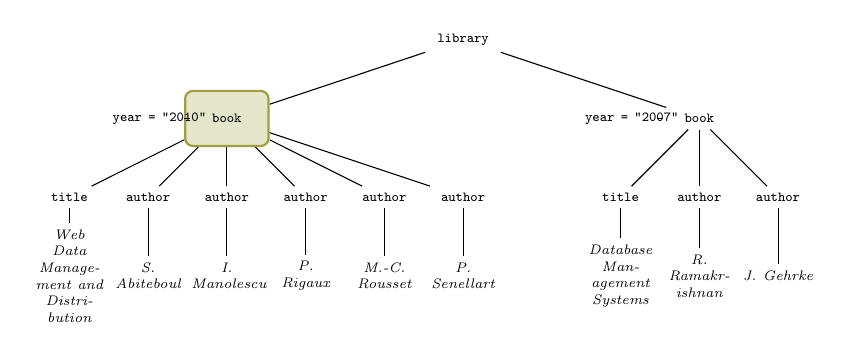
\begin{tikzpicture}[auto]
\tiny
  \tikzstyle{emptyStyle}=[text width=0.9cm, text centered]
  \tikzstyle{red}=[rounded corners=1mm,thick,draw=red!75,fill=red!20,text width=0.9cm, text centered]
  \tikzstyle{DarkViolet}=[rounded corners=1mm,thick,draw=DarkViolet!75,fill=DarkViolet!20,minimum size=7mm,text width=0.8cm, text centered]
  \tikzstyle{green}=[rounded corners=1mm,thick,draw=DarkOliveGreen!75,fill=DarkOliveGreen!20,minimum size=7mm,text width=0.8cm, text centered]
  \tikzstyle{cyan}=[rounded corners=1mm,thick,draw=DarkCyan!75,fill=DarkCyan!20,minimum size=7mm,text width=0.8cm, text centered]
 \tikzstyle{every label}=[black]
  \tikzstyle{HotPink}=[rounded corners=1mm,thick,draw=HotPink!75,fill=HotPink!20,minimum size=7mm,text width=0.8cm, text centered]
  \tikzstyle{noeudcourant}=[rounded corners=1mm,thick,draw=Olive!75,fill=Olive!20,minimum size=7mm,text width=0.9cm, text centered]
  \tikzstyle{indiaRed}=[rounded corners=1mm,thick,draw=indiaRed!75,fill=indiaRed!20,minimum size=7mm,text width=0.9cm, text centered]

  \begin{scope}
   % \node[emptyStyle](r) at (7,5) {Root};  
   %\node[emptyStyle](entete) at (3,4) {\texttt{$<?xml$ version $...>$}};
   %\draw[-] (r) -- (entete);
   \node[emptyStyle](library) at (7,4) {\verb?library?};
   % \draw[-] (r) -- (library);

    \node[noeudcourant](book1) at (4,3) {\verb?book?};
   \draw[-] (library) -- (book1);
   \node[emptyStyle](book2) at (10,3) {\verb?book?};
   \draw[-] (library) -- (book2);

    \node[emptyStyle](year1) at (3,3) {\verb?year = "2010"?};
   \draw[-] (book1) -- (year1);
    \node[emptyStyle](title1) at (2,2) {\verb?title?};
   \draw[-] (book1) -- (title1);
 \node[emptyStyle](texttitle1) at (2,1) {\it Web Data Management and Distribution};
   \draw[-] (title1) -- (texttitle1);
    \node[emptyStyle](author1) at (3,2) {\verb?author?};
   \draw[-] (book1) -- (author1);
   \node[emptyStyle](textauthor1) at (3,1) {\it S. Abiteboul};
   \draw[-] (author1) -- (textauthor1);
    \node[emptyStyle](author2) at (4,2) {\verb?author?};
   \draw[-] (book1) -- (author2);
   \node[emptyStyle](textauthor2) at (4,1) {\it I. Manolescu};
   \draw[-] (author2) -- (textauthor2);
    \node[emptyStyle](author3) at (5,2) {\verb?author?};
   \draw[-] (book1) -- (author3);
   \node[emptyStyle](textauthor3) at (5,1) {\it P. Rigaux};
   \draw[-] (author3) -- (textauthor3);
    \node[emptyStyle](author4) at (6,2) {\verb?author?};
   \draw[-] (book1) -- (author4);
   \node[emptyStyle](textauthor4) at (6,1) {\it M.-C. Rousset};
   \draw[-] (author4) -- (textauthor4);
    \node[emptyStyle](author5) at (7,2) {\verb?author?};
   \draw[-] (book1) -- (author5);
   \node[emptyStyle](textauthor5) at (7,1) {\it P. Senellart};
   \draw[-] (author5) -- (textauthor5);

    \node[emptyStyle](year2) at (9,3) {\verb?year = "2007"?};
   \draw[-] (book2) -- (year2);
    \node[emptyStyle](title2) at (9,2) {\verb?title?};
   \draw[-] (book2) -- (title2);
 \node[emptyStyle](texttitle2) at (9,1) {\it Database Management Systems};
   \draw[-] (title2) -- (texttitle2);
    \node[emptyStyle](author1prime) at (10,2) {\verb?author?};
   \draw[-] (book2) -- (author1prime);
   \node[emptyStyle](textauthor1prime) at (10,1) {\it R. Ramakrishnan};
   \draw[-] (author1prime) -- (textauthor1prime);
    \node[emptyStyle](author2prime) at (11,2) {\verb?author?};
   \draw[-] (book2) -- (author2prime);
   \node[emptyStyle](textauthor2prime) at (11,1) {\it J. Gehrke};
   \draw[-] (author2prime) -- (textauthor2prime);
\end{scope}
\end{tikzpicture}




\end{frame}


 \begin{frame}{Quelques axes en exemple : \texttt{attribute}}
\texttt{attribute} : sélectionne les attributs du n{\oe}ud courant.


\bigskip

\begin{tikzpicture}[auto]
\tiny
  \tikzstyle{emptyStyle}=[text width=0.9cm, text centered]
  \tikzstyle{red}=[rounded corners=1mm,thick,draw=red!75,fill=red!20,text width=0.9cm, text centered]
  \tikzstyle{DarkViolet}=[rounded corners=1mm,thick,draw=DarkViolet!75,fill=DarkViolet!20,minimum size=7mm,text width=0.8cm, text centered]
  \tikzstyle{green}=[rounded corners=1mm,thick,draw=DarkOliveGreen!75,fill=DarkOliveGreen!20,minimum size=7mm,text width=0.8cm, text centered]
  \tikzstyle{cyan}=[rounded corners=1mm,thick,draw=DarkCyan!75,fill=DarkCyan!20,minimum size=7mm,text width=0.8cm, text centered]
 \tikzstyle{every label}=[black]
  \tikzstyle{HotPink}=[rounded corners=1mm,thick,draw=HotPink!75,fill=HotPink!20,minimum size=7mm,text width=0.8cm, text centered]
  \tikzstyle{noeudcourant}=[rounded corners=1mm,thick,draw=Olive!75,fill=Olive!20,minimum size=7mm,text width=0.9cm, text centered]
  \tikzstyle{indiaRed}=[rounded corners=1mm,thick,draw=indiaRed!75,fill=indiaRed!20,minimum size=7mm,text width=0.9cm, text centered]

  \begin{scope}
   % \node[emptyStyle](r) at (7,5) {Root};  
   %\node[emptyStyle](entete) at (3,4) {\texttt{$<?xml$ version $...>$}};
   %\draw[-] (r) -- (entete);
   \node[emptyStyle](library) at (7,4) {\verb?library?};
   % \draw[-] (r) -- (library);

    \node[noeudcourant](book1) at (4,3) {\verb?book?};
   \draw[-] (library) -- (book1);
   \node[emptyStyle](book2) at (10,3) {\verb?book?};
   \draw[-] (library) -- (book2);

    \node[indiaRed](year1) at (3,3) {\verb?year = "2010"?};
   \draw[-] (book1) -- (year1);
    \node[emptyStyle](title1) at (2,2) {\verb?title?};
   \draw[-] (book1) -- (title1);
 \node[emptyStyle](texttitle1) at (2,1) {\it Web Data Management and Distribution};
   \draw[-] (title1) -- (texttitle1);
    \node[emptyStyle](author1) at (3,2) {\verb?author?};
   \draw[-] (book1) -- (author1);
   \node[emptyStyle](textauthor1) at (3,1) {\it S. Abiteboul};
   \draw[-] (author1) -- (textauthor1);
    \node[emptyStyle](author2) at (4,2) {\verb?author?};
   \draw[-] (book1) -- (author2);
   \node[emptyStyle](textauthor2) at (4,1) {\it I. Manolescu};
   \draw[-] (author2) -- (textauthor2);
    \node[emptyStyle](author3) at (5,2) {\verb?author?};
   \draw[-] (book1) -- (author3);
   \node[emptyStyle](textauthor3) at (5,1) {\it P. Rigaux};
   \draw[-] (author3) -- (textauthor3);
    \node[emptyStyle](author4) at (6,2) {\verb?author?};
   \draw[-] (book1) -- (author4);
   \node[emptyStyle](textauthor4) at (6,1) {\it M.-C. Rousset};
   \draw[-] (author4) -- (textauthor4);
    \node[emptyStyle](author5) at (7,2) {\verb?author?};
   \draw[-] (book1) -- (author5);
   \node[emptyStyle](textauthor5) at (7,1) {\it P. Senellart};
   \draw[-] (author5) -- (textauthor5);

    \node[emptyStyle](year2) at (9,3) {\verb?year = "2007"?};
   \draw[-] (book2) -- (year2);
    \node[emptyStyle](title2) at (9,2) {\verb?title?};
   \draw[-] (book2) -- (title2);
 \node[emptyStyle](texttitle2) at (9,1) {\it Database Management Systems};
   \draw[-] (title2) -- (texttitle2);
    \node[emptyStyle](author1prime) at (10,2) {\verb?author?};
   \draw[-] (book2) -- (author1prime);
   \node[emptyStyle](textauthor1prime) at (10,1) {\it R. Ramakrishnan};
   \draw[-] (author1prime) -- (textauthor1prime);
    \node[emptyStyle](author2prime) at (11,2) {\verb?author?};
   \draw[-] (book2) -- (author2prime);
   \node[emptyStyle](textauthor2prime) at (11,1) {\it J. Gehrke};
   \draw[-] (author2prime) -- (textauthor2prime);
\end{scope}
\end{tikzpicture}

\end{frame}



\begin{frame}[allowframebreaks]{Exemple}

%\begin{center}
%\begin{minipage}{0.7\textwidth}
%\lstinputlisting[basicstyle=\tiny, language=XML,breaklines=true, caption={Un simple fichier XML}]{codes/livresExXpath.xml}
%\end{minipage}
%\end{center}

%\framebreak

\texttt{/child::library/child::*/@year}

\medskip

S'abrège en\,: \texttt{/library/*/@year}

\begin{center}
\begin{tikzpicture}[auto]
\tiny
  \tikzstyle{emptyStyle}=[text width=0.9cm, text centered]
  \tikzstyle{parser}=[rounded corners=3mm,thick,draw=DarkViolet!75,fill=DarkViolet!20,,text centered]
  \tikzstyle{appli}=[rounded corners=1mm,thick,draw=red!75,fill=red!20,text centered,text width=2cm]
  \tikzstyle{every label}=[black]

  \begin{scope}
    \node[emptyStyle](r) at (6,5) {Root};
   \node[emptyStyle](comment) at (1,4) {\texttt{\verb?<!-- ceci ... >?}};
   \draw[-] (r) -- (comment);
    %\node[emptyStyle](entete) at (3,4) {\texttt{$<?xml$ version $...>$}};
   %\draw[-] (r) -- (entete);
    \node[emptyStyle](library) at (6,4) {\verb?<library> ... </library>?};
   \draw[-] (r) -- (library);

    \node[emptyStyle](book1) at (3,3) {\verb?<book> ... </book>?};
   \draw[-] (library) -- (book1);
    \node[emptyStyle](book2) at (6,3) {\verb?<book> ... </book>?};
   \draw[-] (library) -- (book2);
    \node[emptyStyle](book3) at (10,3) {\verb?<book> ... </book>?};
   \draw[-] (library) -- (book3);

    \node[emptyStyle](year1) at (2,3) {\verb?year = "1857"?};
   \draw[-] (book1) -- (year1);
    \node[emptyStyle](author1) at (2,2) {\verb?<author> ... </author>?};
   \draw[-] (book1) -- (author1);
    \node[emptyStyle](textauthor1) at (2,1) {\it Charles Baudelaire};
   \draw[-] (author1) -- (textauthor1);
    \node[emptyStyle](title1) at (3,2) {\verb?<title> ... </title>?};
   \draw[-] (book1) -- (title1);
    \node[emptyStyle](texttitle1) at (3,1) {\it Les fleurs du mal};
   \draw[-] (title1) -- (texttitle1);

    \node[emptyStyle](year2) at (5,3) {\verb?year = "1862"?};
   \draw[-] (book2) -- (year2);
    \node[emptyStyle](author2) at (6,2) {\verb?<author> ... </author>?};
   \draw[-] (book2) -- (author2);
    \node[emptyStyle](textauthor2) at (6,1) {\it Victor Hugo};
   \draw[-] (author2) -- (textauthor2);
    \node[emptyStyle](ln2) at (5,2) {\verb?ln = "Besancon"?};
   \draw[-] (author2) -- (ln2);
    \node[emptyStyle](title2) at (7,2) {\verb?<title> ... </title>?};
   \draw[-] (book2) -- (title2);
    \node[emptyStyle](texttitle2) at (7,1) {\it Les miserables};
   \draw[-] (title2) -- (texttitle2);

    \node[emptyStyle](year3) at (9,3) {\verb?year = "1877"?};
   \draw[-] (book3) -- (year3);
    \node[emptyStyle](author3) at (10,2) {\verb?<author> ... </author>?};
   \draw[-] (book3) -- (author3);
    \node[emptyStyle](textauthor3) at (10,1) {\it Emile Zola};
   \draw[-] (author3) -- (textauthor3);
    \node[emptyStyle](ln3) at (9,2) {\verb?ln = "Paris"?};
   \draw[-] (author3) -- (ln3);
    \node[emptyStyle](title3) at (11,2) {\verb?<title> ... </title>?};
   \draw[-] (book3) -- (title3);
    \node[emptyStyle](texttitle3) at (11,1) {\it L'assomoir};
   \draw[-] (title3) -- (texttitle3);

\end{scope}

%  \begin{pgfonlayer}{background}
%    \filldraw [line width=4mm,join=round,black!20]
%      (parser.north  -| parser.west)  rectangle (serial.south  -| serial.east);
%\end{pgfonlayer}


\end{tikzpicture}
\end{center}

\framebreak

\texttt{\textcolor{red}{\bf /}library/*/@year}

\begin{center}
\begin{tikzpicture}[auto]
\tiny
  \tikzstyle{emptyStyle}=[text width=0.9cm, text centered]
  \tikzstyle{red}=[rounded corners=1mm,thick,draw=red!75,fill=red!20,text width=0.9cm, text centered]
  \tikzstyle{DarkViolet}=[rounded corners=1mm,thick,draw=DarkViolet!75,fill=DarkViolet!20,minimum size=7mm,text width=0.8cm, text centered]
 \tikzstyle{every label}=[black]

  \begin{scope}
    \node[red](r) at (6,5) {Root};
   \node[emptyStyle](comment) at (1,4) {\texttt{\verb?<!-- ceci ... >?}};
   \draw[-] (r) -- (comment);
    %\node[emptyStyle](entete) at (3,4) {\texttt{$<?xml$ version $...>$}};
   %\draw[-] (r) -- (entete);
    \node[emptyStyle](library) at (6,4) {\verb?<library> ... </library>?};
   \draw[-] (r) -- (library);

    \node[emptyStyle](book1) at (3,3) {\verb?<book> ... </book>?};
   \draw[-] (library) -- (book1);
    \node[emptyStyle](book2) at (6,3) {\verb?<book> ... </book>?};
   \draw[-] (library) -- (book2);
    \node[emptyStyle](book3) at (10,3) {\verb?<book> ... </book>?};
   \draw[-] (library) -- (book3);

    \node[emptyStyle](year1) at (2,3) {\verb?year = "1857"?};
   \draw[-] (book1) -- (year1);
    \node[emptyStyle](author1) at (2,2) {\verb?<author> ... </author>?};
   \draw[-] (book1) -- (author1);
    \node[emptyStyle](textauthor1) at (2,1) {\it Charles Baudelaire};
   \draw[-] (author1) -- (textauthor1);
    \node[emptyStyle](title1) at (3,2) {\verb?<title> ... </title>?};
   \draw[-] (book1) -- (title1);
    \node[emptyStyle](texttitle1) at (3,1) {\it Les fleurs du mal};
   \draw[-] (title1) -- (texttitle1);

    \node[emptyStyle](year2) at (5,3) {\verb?year = "1862"?};
   \draw[-] (book2) -- (year2);
    \node[emptyStyle](author2) at (6,2) {\verb?<author> ... </author>?};
   \draw[-] (book2) -- (author2);
    \node[emptyStyle](textauthor2) at (6,1) {\it Victor Hugo};
   \draw[-] (author2) -- (textauthor2);
    \node[emptyStyle](ln2) at (5,2) {\verb?ln = "Besancon"?};
   \draw[-] (author2) -- (ln2);
    \node[emptyStyle](title2) at (7,2) {\verb?<title> ... </title>?};
   \draw[-] (book2) -- (title2);
    \node[emptyStyle](texttitle2) at (7,1) {\it Les miserables};
   \draw[-] (title2) -- (texttitle2);

    \node[emptyStyle](year3) at (9,3) {\verb?year = "1877"?};
   \draw[-] (book3) -- (year3);
    \node[emptyStyle](author3) at (10,2) {\verb?<author> ... </author>?};
   \draw[-] (book3) -- (author3);
    \node[emptyStyle](textauthor3) at (10,1) {\it Emile Zola};
   \draw[-] (author3) -- (textauthor3);
    \node[emptyStyle](ln3) at (9,2) {\verb?ln = "Paris"?};
   \draw[-] (author3) -- (ln3);
    \node[emptyStyle](title3) at (11,2) {\verb?<title> ... </title>?};
   \draw[-] (book3) -- (title3);
    \node[emptyStyle](texttitle3) at (11,1) {\it L'assomoir};
   \draw[-] (title3) -- (texttitle3);

\end{scope}

%  \begin{pgfonlayer}{background}
%    \filldraw [line width=4mm,join=round,black!20]
%      (parser.north  -| parser.west)  rectangle (serial.south  -| serial.east);
%\end{pgfonlayer}


\end{tikzpicture}
\end{center}


\framebreak

\texttt{\textcolor{red}{\bf /}\textcolor{DarkViolet}{\bf library}/*/@year}

\begin{center}
\begin{tikzpicture}[auto]
\tiny
  \tikzstyle{emptyStyle}=[text width=0.9cm, text centered]
  \tikzstyle{red}=[rounded corners=1mm,thick,draw=red!75,fill=red!20,text width=0.9cm, text centered]
  \tikzstyle{DarkViolet}=[rounded corners=1mm,thick,draw=DarkViolet!75,fill=DarkViolet!20,minimum size=7mm,text width=0.8cm, text centered]
 \tikzstyle{every label}=[black]

  \begin{scope}
    \node[red](r) at (6,5) {Root};
   \node[emptyStyle](comment) at (1,4) {\texttt{\verb?<!-- ceci ... >?}};
   \draw[-] (r) -- (comment);
    %\node[emptyStyle](entete) at (3,4) {\texttt{$<?xml$ version $...>$}};
   %\draw[-] (r) -- (entete);
    \node[DarkViolet](library) at (6,4) {\verb?<library> ... </library>?};
   \draw[-] (r) -- (library);

    \node[emptyStyle](book1) at (3,3) {\verb?<book> ... </book>?};
   \draw[-] (library) -- (book1);
    \node[emptyStyle](book2) at (6,3) {\verb?<book> ... </book>?};
   \draw[-] (library) -- (book2);
    \node[emptyStyle](book3) at (10,3) {\verb?<book> ... </book>?};
   \draw[-] (library) -- (book3);

    \node[emptyStyle](year1) at (2,3) {\verb?year = "1857"?};
   \draw[-] (book1) -- (year1);
    \node[emptyStyle](author1) at (2,2) {\verb?<author> ... </author>?};
   \draw[-] (book1) -- (author1);
    \node[emptyStyle](textauthor1) at (2,1) {\it Charles Baudelaire};
   \draw[-] (author1) -- (textauthor1);
    \node[emptyStyle](title1) at (3,2) {\verb?<title> ... </title>?};
   \draw[-] (book1) -- (title1);
    \node[emptyStyle](texttitle1) at (3,1) {\it Les fleurs du mal};
   \draw[-] (title1) -- (texttitle1);

    \node[emptyStyle](year2) at (5,3) {\verb?year = "1862"?};
   \draw[-] (book2) -- (year2);
    \node[emptyStyle](author2) at (6,2) {\verb?<author> ... </author>?};
   \draw[-] (book2) -- (author2);
    \node[emptyStyle](textauthor2) at (6,1) {\it Victor Hugo};
   \draw[-] (author2) -- (textauthor2);
    \node[emptyStyle](ln2) at (5,2) {\verb?ln = "Besancon"?};
   \draw[-] (author2) -- (ln2);
    \node[emptyStyle](title2) at (7,2) {\verb?<title> ... </title>?};
   \draw[-] (book2) -- (title2);
    \node[emptyStyle](texttitle2) at (7,1) {\it Les miserables};
   \draw[-] (title2) -- (texttitle2);

    \node[emptyStyle](year3) at (9,3) {\verb?year = "1877"?};
   \draw[-] (book3) -- (year3);
    \node[emptyStyle](author3) at (10,2) {\verb?<author> ... </author>?};
   \draw[-] (book3) -- (author3);
    \node[emptyStyle](textauthor3) at (10,1) {\it Emile Zola};
   \draw[-] (author3) -- (textauthor3);
    \node[emptyStyle](ln3) at (9,2) {\verb?ln = "Paris"?};
   \draw[-] (author3) -- (ln3);
    \node[emptyStyle](title3) at (11,2) {\verb?<title> ... </title>?};
   \draw[-] (book3) -- (title3);
    \node[emptyStyle](texttitle3) at (11,1) {\it L'assomoir};
   \draw[-] (title3) -- (texttitle3);

\end{scope}

%  \begin{pgfonlayer}{background}
%    \filldraw [line width=4mm,join=round,black!20]
%      (parser.north  -| parser.west)  rectangle (serial.south  -| serial.east);
%\end{pgfonlayer}


\end{tikzpicture}
\end{center}

\framebreak

\texttt{\textcolor{red}{\bf /}\textcolor{DarkViolet}{\bf library}\textcolor{DarkOliveGreen}{\bf /*}/@year}

\begin{center}
\begin{tikzpicture}[auto]
\tiny
  \tikzstyle{emptyStyle}=[text width=0.9cm, text centered]
  \tikzstyle{red}=[rounded corners=1mm,thick,draw=red!75,fill=red!20,text width=0.9cm, text centered]
  \tikzstyle{DarkViolet}=[rounded corners=1mm,thick,draw=DarkViolet!75,fill=DarkViolet!20,minimum size=7mm,text width=0.8cm, text centered]
  \tikzstyle{green}=[rounded corners=1mm,thick,draw=DarkOliveGreen!75,fill=DarkOliveGreen!20,minimum size=7mm,text width=0.8cm, text centered]
 \tikzstyle{every label}=[black]

  \begin{scope}
    \node[red](r) at (6,5) {Root};
   \node[emptyStyle](comment) at (1,4) {\texttt{\verb?<!-- ceci ... >?}};
   \draw[-] (r) -- (comment);
    %\node[emptyStyle](entete) at (3,4) {\texttt{$<?xml$ version $...>$}};
   %\draw[-] (r) -- (entete);
    \node[DarkViolet](library) at (6,4) {\verb?<library> ... </library>?};
   \draw[-] (r) -- (library);

    \node[green](book1) at (3,3) {\verb?<book> ... </book>?};
   \draw[-] (library) -- (book1);
    \node[green](book2) at (6,3) {\verb?<book> ... </book>?};
   \draw[-] (library) -- (book2);
    \node[green](book3) at (10,3) {\verb?<book> ... </book>?};
   \draw[-] (library) -- (book3);

    \node[emptyStyle](year1) at (2,3) {\verb?year = "1857"?};
   \draw[-] (book1) -- (year1);
    \node[emptyStyle](author1) at (2,2) {\verb?<author> ... </author>?};
   \draw[-] (book1) -- (author1);
    \node[emptyStyle](textauthor1) at (2,1) {\it Charles Baudelaire};
   \draw[-] (author1) -- (textauthor1);
    \node[emptyStyle](title1) at (3,2) {\verb?<title> ... </title>?};
   \draw[-] (book1) -- (title1);
    \node[emptyStyle](texttitle1) at (3,1) {\it Les fleurs du mal};
   \draw[-] (title1) -- (texttitle1);

    \node[emptyStyle](year2) at (5,3) {\verb?year = "1862"?};
   \draw[-] (book2) -- (year2);
    \node[emptyStyle](author2) at (6,2) {\verb?<author> ... </author>?};
   \draw[-] (book2) -- (author2);
    \node[emptyStyle](textauthor2) at (6,1) {\it Victor Hugo};
   \draw[-] (author2) -- (textauthor2);
    \node[emptyStyle](ln2) at (5,2) {\verb?ln = "Besancon"?};
   \draw[-] (author2) -- (ln2);
    \node[emptyStyle](title2) at (7,2) {\verb?<title> ... </title>?};
   \draw[-] (book2) -- (title2);
    \node[emptyStyle](texttitle2) at (7,1) {\it Les miserables};
   \draw[-] (title2) -- (texttitle2);

    \node[emptyStyle](year3) at (9,3) {\verb?year = "1877"?};
   \draw[-] (book3) -- (year3);
    \node[emptyStyle](author3) at (10,2) {\verb?<author> ... </author>?};
   \draw[-] (book3) -- (author3);
    \node[emptyStyle](textauthor3) at (10,1) {\it Emile Zola};
   \draw[-] (author3) -- (textauthor3);
    \node[emptyStyle](ln3) at (9,2) {\verb?ln = "Paris"?};
   \draw[-] (author3) -- (ln3);
    \node[emptyStyle](title3) at (11,2) {\verb?<title> ... </title>?};
   \draw[-] (book3) -- (title3);
    \node[emptyStyle](texttitle3) at (11,1) {\it L'assomoir};
   \draw[-] (title3) -- (texttitle3);

\end{scope}

%  \begin{pgfonlayer}{background}
%    \filldraw [line width=4mm,join=round,black!20]
%      (parser.north  -| parser.west)  rectangle (serial.south  -| serial.east);
%\end{pgfonlayer}


\end{tikzpicture}
\end{center}


\framebreak

\texttt{\textcolor{red}{\bf /}\textcolor{DarkViolet}{\bf library}\textcolor{DarkOliveGreen}{\bf /*}\textcolor{DarkCyan}{\bf  /@year}}


\begin{center}
\begin{tikzpicture}[auto]
\tiny
  \tikzstyle{emptyStyle}=[text width=0.9cm, text centered]
  \tikzstyle{red}=[rounded corners=1mm,thick,draw=red!75,fill=red!20,text width=0.9cm, text centered]
  \tikzstyle{DarkViolet}=[rounded corners=1mm,thick,draw=DarkViolet!75,fill=DarkViolet!20,minimum size=7mm,text width=0.8cm, text centered]
  \tikzstyle{green}=[rounded corners=1mm,thick,draw=DarkOliveGreen!75,fill=DarkOliveGreen!20,minimum size=7mm,text width=0.8cm, text centered]
  \tikzstyle{cyan}=[rounded corners=1mm,thick,draw=DarkCyan!75,fill=DarkCyan!20,minimum size=7mm,text width=0.8cm, text centered]
 \tikzstyle{every label}=[black]

  \begin{scope}
    \node[red](r) at (6,5) {Root};
   \node[emptyStyle](comment) at (1,4) {\texttt{\verb?<!-- ceci ... >?}};
   \draw[-] (r) -- (comment);
    %\node[emptyStyle](entete) at (3,4) {\texttt{$<?xml$ version $...>$}};
   %\draw[-] (r) -- (entete);
    \node[DarkViolet](library) at (6,4) {\verb?<library> ... </library>?};
   \draw[-] (r) -- (library);

    \node[green](book1) at (3,3) {\verb?<book> ... </book>?};
   \draw[-] (library) -- (book1);
    \node[green](book2) at (6,3) {\verb?<book> ... </book>?};
   \draw[-] (library) -- (book2);
    \node[green](book3) at (10,3) {\verb?<book> ... </book>?};
   \draw[-] (library) -- (book3);

    \node[cyan](year1) at (2,3) {\verb?year = "1857"?};
   \draw[-] (book1) -- (year1);
    \node[emptyStyle](author1) at (2,2) {\verb?<author> ... </author>?};
   \draw[-] (book1) -- (author1);
    \node[emptyStyle](textauthor1) at (2,1) {\it Charles Baudelaire};
   \draw[-] (author1) -- (textauthor1);
    \node[emptyStyle](title1) at (3,2) {\verb?<title> ... </title>?};
   \draw[-] (book1) -- (title1);
    \node[emptyStyle](texttitle1) at (3,1) {\it Les fleurs du mal};
   \draw[-] (title1) -- (texttitle1);

    \node[cyan](year2) at (5,3) {\verb?year = "1862"?};
   \draw[-] (book2) -- (year2);
    \node[emptyStyle](author2) at (6,2) {\verb?<author> ... </author>?};
   \draw[-] (book2) -- (author2);
    \node[emptyStyle](textauthor2) at (6,1) {\it Victor Hugo};
   \draw[-] (author2) -- (textauthor2);
    \node[emptyStyle](ln2) at (5,2) {\verb?ln = "Besancon"?};
   \draw[-] (author2) -- (ln2);
    \node[emptyStyle](title2) at (7,2) {\verb?<title> ... </title>?};
   \draw[-] (book2) -- (title2);
    \node[emptyStyle](texttitle2) at (7,1) {\it Les miserables};
   \draw[-] (title2) -- (texttitle2);

    \node[cyan](year3) at (9,3) {\verb?year = "1877"?};
   \draw[-] (book3) -- (year3);
    \node[emptyStyle](author3) at (10,2) {\verb?<author> ... </author>?};
   \draw[-] (book3) -- (author3);
    \node[emptyStyle](textauthor3) at (10,1) {\it Emile Zola};
   \draw[-] (author3) -- (textauthor3);
    \node[emptyStyle](ln3) at (9,2) {\verb?ln = "Paris"?};
   \draw[-] (author3) -- (ln3);
    \node[emptyStyle](title3) at (11,2) {\verb?<title> ... </title>?};
   \draw[-] (book3) -- (title3);
    \node[emptyStyle](texttitle3) at (11,1) {\it L'assomoir};
   \draw[-] (title3) -- (texttitle3);

\end{scope}

%  \begin{pgfonlayer}{background}
%    \filldraw [line width=4mm,join=round,black!20]
%      (parser.north  -| parser.west)  rectangle (serial.south  -| serial.east);
%\end{pgfonlayer}


\end{tikzpicture}
\end{center}

\end{frame}

\section{Tests et prédicats}


\subsection{Test de n{\oe}ud}

\begin{frame}{Les tests de n{\oe}uds}

Test du type du n{\oe}ud :
\begin{description}
\item[\verb?node()?] sélectionne les nœuds quelque soit leur ``type'' (élément, n{\oe}ud texte, processing-instruction)
\item[\verb?text()?] sélectionne les n{\oe}uds de ``type'' texte
\item[\verb?comment()?] sélectionne les nœuds de ``type'' commentaire
\item[\verb?processing-instruction()?] sélectionne les nœuds de ``type'' proc-instruction
\end{description}

\medskip

Test de nom :
\begin{description}
\item[\verb?name?] sélectionne les éléments ou attributs de noms \texttt{name}
\item[\verb?*?] sélectionne les n{\oe}uds \alert{nommés} (\domtype{Element} ou \domtype{Attribute}), quel que soit le nom.
\end{description}

\end{frame}

\begin{frame}{Expressions complètes avec \texttt{child}}
Revenons sur \texttt{child}.

\begin{description}
\item[\verb?child::para?] sélectionne l'élément de nom \texttt{para}, enfant du n{\oe}ud courant. 

\item[\verb?child::*?] sélectionne tous les \domtype{Elements} enfants du n{\oe}ud courant (pas les n{\oe}uds \domtype{Text}). 

\item[\verb?child::text()?] sélectionne tous les n{\oe}uds \domtype{Text} enfants du n{\oe}ud courant.

\item[\verb?child::node()?] sélectionne tous les \domtype{Elements} enfants du n{\oe}ud courant, quel que soit leur type.
\end{description}


\end{frame}



\begin{frame}{Mise en jambe}

\begin{small}
\prof{A faire sous baseX car zrinity renvoie des résultats difficiles à interpréter.}

\begin{exoblock}
Que ``cherchent'' à calculer les expressions suivantes ? Donner les résultats de leurs évaluations sur le fichier \textit{twobooks.xml}.\\

\verb?/child::library?

\verb?/child::*/child::book/child::title/child::text()? \prof{Deux résultats de type text Web Data Management Distribution et Database Management Systems}

\verb?/child::library/child::book/attribute::*?	\prof{tous les attributs -qq leur nom- des books)}

\verb?/child::library/child::book/attribute::year?	\prof{tous les attributs -year des books)}

\verb?/descendant::author? \prof{tous les auteurs du doc ici}

%\verb?/descendant::*[ancestor::book]? \prof{dans tous les noeuds de l'arbre, ceux qui ont un ancetre book donc les title et les authors}

\verb?/child::*/descendant::library? \prof{personne car on descend qur library pour on cherche un secendant library (aurait renvoyé library siça avait été un descendant or self)}

\verb?/descendant::book/child::title? \prof{descend sur les book puis leur title}

\end{exoblock}

\end{small}


\end{frame}


\subsection{Les prédicats}

\begin{frame}{Les prédicats}

Un prédicat est une condition filtrant un ensemble contexte (ne garde que les n{\oe}uds (sous-arbres) satisfaisant la condition).\\

\medskip


Contraintes booléennes (combinaison logique (and, or, not) de contraintes plus simples) :
\begin{itemize}
\item Comparaisons \\
	\verb?child::biblio/child::livre[attribute::ISBN='0\-262\-01210-3']/child::authors?
\item Existence d'un attribut ou d'un élément \\
	\verb?document[child::date]?\\
	\verb?personne[attribute::date\_naissance]?
\end{itemize}


\bigskip

Exemples (W3C) :\\

\smallskip

\verb?child::employee[child::secretary or child::assistant]?\\

\smallskip

\verb?descendant::toy[not(attribute::color = "red") and attribute::country= "China"]?

\end{frame}


\begin{frame}{Evaluation des prédicats}

Une petite subtilité...

\begin{itemize}
\item Si l'expression est une ``véritable'' expression booléenne, pas de soucis\\
\textcolor{cyan}{\verb?/inventory/drink/lemonade[child::amount>15]?}
\item Si le résultat du prédicat ou si le prédicat est un nombre, le résultat du prédicat est converti à true si le nombre est égal à la position dans le contexte d'évaluation (sinon false)\\
Ainsi, \textcolor{cyan}{\verb?para[3]?} est équivalent à \textcolor{cyan}{\verb?para[position()=3]?}.
\end{itemize}
\end{frame}

\begin{frame}{Zoom sur les prédicats utilisant la fonction \texttt{position()} }


\begin{center}
\begin{minipage}{0.7\textwidth}
\lstinputlisting[firstline=2,basicstyle=\tiny, label=twobooks, language=XML,breaklines=true, caption={Extrait de twobooks.xml}]{codes/twobooks.xml}
\end{minipage}
\end{center}


\only<1>{
\begin{exampleblock}{Example}
\verb?/child::library/child::book/child::author[position()=1]? 
%\prof{sélectionne le premier auteur (le premier fils \verb?author?) para du n{\oe}ud contextuel}

\prof{Résultat :\\ \prof{exo: dessiner arbre. Rmq : title ``sauté'' puisque pas un auteur}
\verb?<author>S. Abiteboul</author>?\\
\verb?<author>R. Ramakrishnan</author>?  
}
\end{exampleblock}
}


\only<2>{
\begin{exampleblock}{Example}
\verb?/child::library/child::book/child::author[position()=last()] ?	 
%\prof{sélectionne le dernier auteur de chaque contexte (de chaque livre).}
\prof{Résultat :\\
\verb?<author>M. Senellart</author>?\\
\verb?<author>J. Gehrke</author>? }
\end{exampleblock}
}

\only<3>{
\begin{exampleblock}{Example}
\verb?/child::library/child::book/child::author[position()=3] ?
%\prof{sélectionne le troisiéme fils auteur du n{\oe}ud contexte (de chaque livre).}
\prof{Résultat :\\
\verb?<author>P. Rigaux</author>?}
\end{exampleblock}
}

\only<4>{
\begin{exampleblock}{Example}
\verb?/child::library/child::book[position()=2]/child::author ?
%\prof{sélectionne le premier auteur de chaque contexte (de chaque livre).}
\prof{Résultat:\\
\verb?<author>R. Ramakrishnan</author>?\\ 
\verb?<author>J. Gehrke</author>? }
\end{exampleblock}
}

\only<5>{
\begin{exampleblock}{Example}
\verb?/child::library/child::book/child::*[position()=1] ?
%\prof{sélectionne le premier fils de chaque contexte (de chaque livre).}
\prof{Résultat :\\
\verb?<title>Web Data Management and Distribution</title>?\\
\verb?<title>Database Management Systems</title>?
}
\end{exampleblock}
}


\only<1-5>
{
\begin{exoblock}
Quel est le résultat de l'évaluation de cette requête appliquée au document \textit{twobooks.xml} ?
\end{exoblock}
}

\end{frame}
